\section{Technik als Deutungsangebot – Raketentechnik und Raumfahrt}

\subsection{Einführung: Technik als historisches Deutungsangebot}

Die Vorlesung betrachtet Raketentechnik nicht primär als technische Entwicklung,
sondern als historisches und gesellschaftliches Deutungsangebot.

Technik besitzt keine feste Bedeutung.
Je nach historischem Kontext kann dieselbe Technologie unterschiedliche Funktionen,
Ziele und Symboliken erhalten.

Zentrale Leitfragen:

\begin{itemize}
    \item Welche Bedeutungen werden Raketen zugeschrieben?
    \item Welche Rolle spielt Krieg bei technischen Innovationen?
    \item Wie verändert sich die Wahrnehmung von Raumfahrt im Laufe der Zeit?
    \item Welche politischen und gesellschaftlichen Interessen prägen technische Entwicklungen?
\end{itemize}

Die Geschichte der Raumfahrt ist daher nicht nur Technikgeschichte,
sondern auch Politik-, Militär- und Kulturgeschichte.

\subsection{Historische Perspektive und Anachronismus}

Zu Beginn wird vor einer häufigen Falle historischer Betrachtung gewarnt:
dem Anachronismus.

Historische Ereignisse werden oft aus heutiger Perspektive bewertet.
Für eine wissenschaftliche Analyse ist jedoch entscheidend, die Sichtweise
der damaligen Akteure und ihren historischen Kontext zu berücksichtigen.

Vergangene Entscheidungen dürfen daher nicht anhand späterer Entwicklungen
oder heutigen Wissens beurteilt werden.

\subsection{Grundlagen der Raketentechnik}

Die technischen Grundprinzipien der Rakete sind erstaunlich konstant geblieben.

Bereits im China des 13. Jahrhunderts wurden Raketen nach dem Rückstossprinzip eingesetzt.

Historisch verändert haben sich jedoch:

\begin{itemize}
    \item Materialien (Stahl, Titan, Nickellegierungen, Carbon)
    \item Antriebssysteme (Feststoff-, Flüssig- und Methantriebwerke)
    \item Steuerungssysteme (digitale Navigation seit den Apollo-Missionen)
    \item Einsatzgebiete und Zwecke
\end{itemize}

Die gleiche Grundtechnologie kann als Waffe,
Trägerrakete, Satellitensystem oder Raumfahrzeug dienen.

\subsection{Technik und Krieg: Die A4 bzw. V2-Rakete}

Ein entscheidender Entwicklungsschritt erfolgte im Zweiten Weltkrieg.

Die Aggregat 4 (A4), später als V2 („Vergeltungswaffe 2“) bezeichnet,
gilt als erste funktionsfähige Fernrakete.

Wichtige Eckpunkte:

\begin{itemize}
    \item Entwicklung unter Wernher von Braun ab 1939
    \item Erste erfolgreiche Tests 1942
    \item Serienproduktion ab 1943
    \item Einsatz gegen Städte wie London und Antwerpen
\end{itemize}

Die Produktion erfolgte in grossen Teilen durch KZ-Häftlinge.
Tausende Menschen wurden zur Arbeit gezwungen,
viele verloren dabei ihr Leben.

Die Geschichte der Rakete ist daher untrennbar mit
nationalsozialistischer Gewalt und Zwangsarbeit verbunden.

\begin{center}
    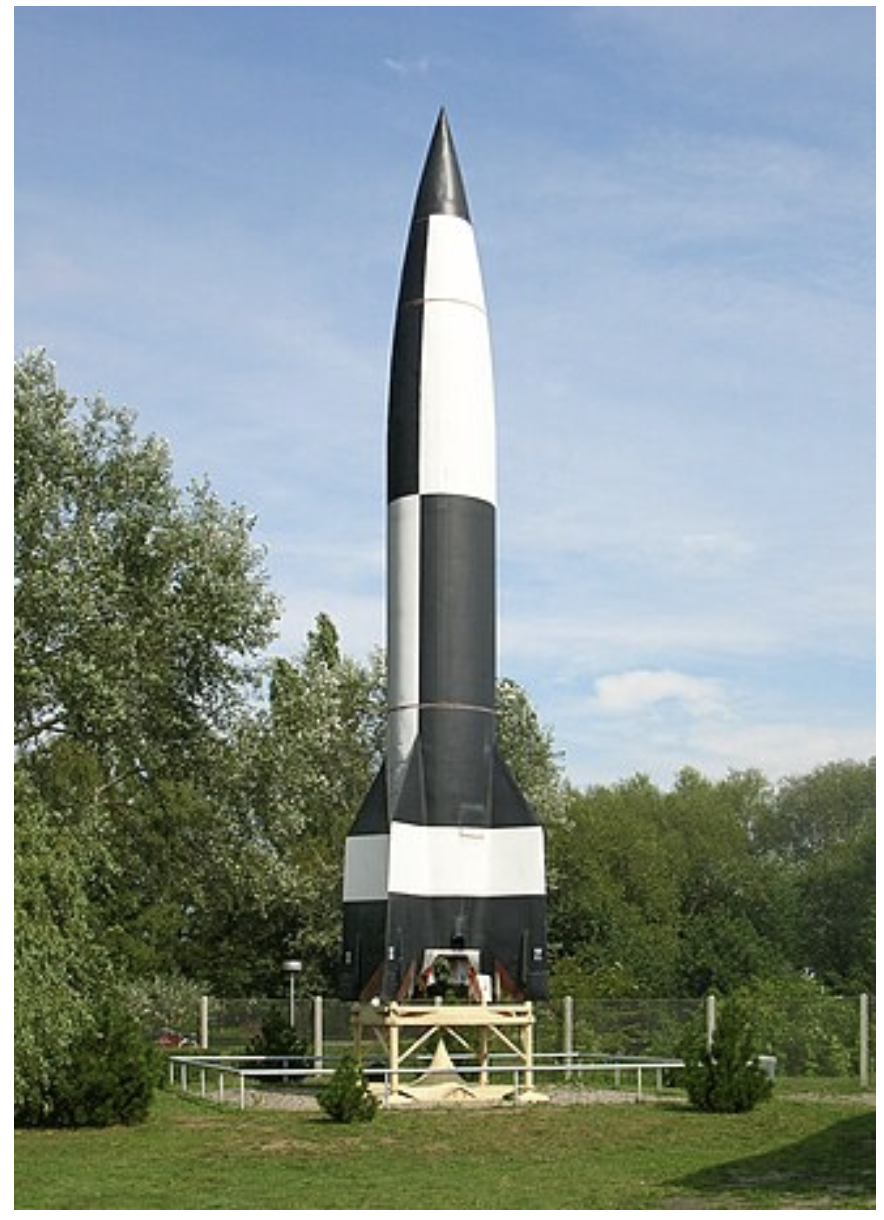
\includegraphics[width=0.8\linewidth]{images/rakete.png}
\end{center}


\subsection{Krieg als Motor technischer Entwicklung?}

Die Vorlesung diskutiert die verbreitete These,
dass Kriege technische Innovationen beschleunigen.

Argumente dafür:

\begin{itemize}
    \item Enorme finanzielle Ressourcen
    \item Enge Zusammenarbeit zwischen Militär, Wissenschaft und Industrie
    \item Hohe politische Priorität
\end{itemize}

Gleichzeitig zeigt sich, dass Krieg Innovationen auch behindern kann:

\begin{itemize}
    \item Geheimhaltung verhindert Wissensaustausch
    \item Fehlender Kostendruck reduziert Effizienz
    \item Produktion und Weiterentwicklung konkurrieren miteinander
    \item Ethische Folgen werden ausgeblendet
\end{itemize}

Die Vorstellung, Krieg sei automatisch ein Innovationstreiber,
wird daher kritisch hinterfragt.

\subsection{Techniker nach dem Zweiten Weltkrieg}

\begin{center}
    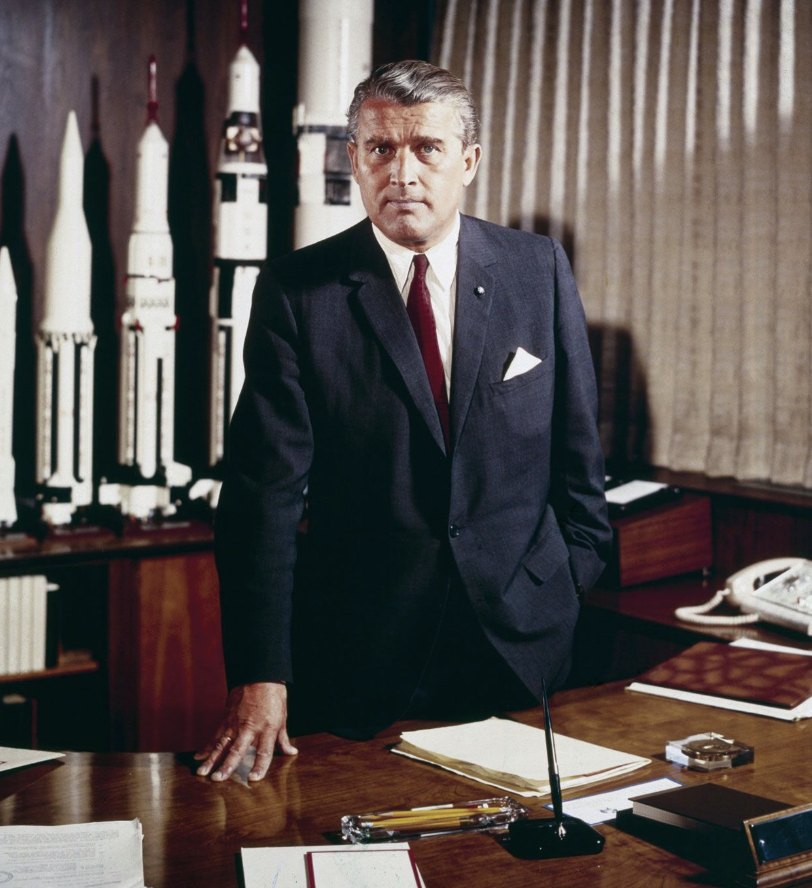
\includegraphics[width=0.8\linewidth]{images/von_Braun.png}
\end{center}

Nach Kriegsende versuchten die Siegermächte,
deutsches Raketenwissen für sich zu nutzen.

Die wichtigsten Programme waren:

\paragraph{Project Paperclip}

Die USA rekrutierten hunderte deutsche Wissenschaftler,
darunter Wernher von Braun.

Viele von ihnen arbeiteten später an den amerikanischen
Raumfahrtprogrammen und den Saturn-Raketen der NASA.

\paragraph{Aktion Ossawakim}

Die Sowjetunion überführte ebenfalls zahlreiche deutsche Spezialisten
in die UdSSR, teilweise freiwillig,
teilweise unter erheblichem Druck.

Damit wurde die deutsche Raketentechnik zu einer wichtigen Grundlage
des späteren Wettlaufs ins All.

\textbf{Bild einfügen:}
Wernher von Braun (wie auf Folie 10).

\subsection{Raumfahrt im Kalten Krieg}

\begin{center}
    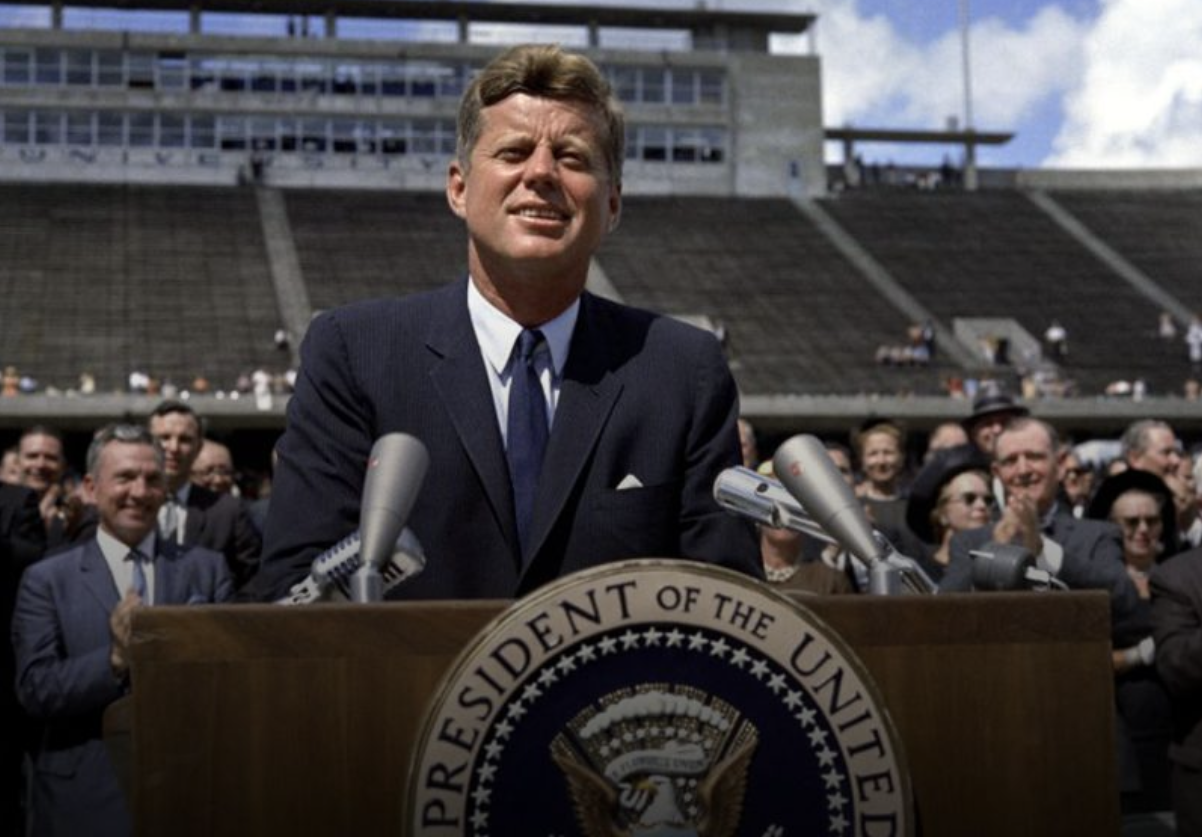
\includegraphics[width=0.8\linewidth]{images/JFK.png}
\end{center}

Im Kalten Krieg wurde Raumfahrt zu einem Symbol
gesellschaftlicher und technologischer Überlegenheit.

Die USA und die Sowjetunion konkurrierten nicht nur militärisch,
sondern auch auf wissenschaftlicher und symbolischer Ebene.

Wichtige Ereignisse:

\begin{itemize}
    \item 1957: Sputnik-Schock
    \item Gründung der NASA
    \item 1961: Juri Gagarin als erster Mensch im Weltall
    \item 1969: Mondlandung der Apollo-11-Mission
\end{itemize}

Raumfahrt wurde zu einem globalen Medienereignis
und zum sichtbaren Ausdruck nationaler Leistungsfähigkeit.

\paragraph{John F. Kennedys Mondrede}

Die Rede „We choose to go to the moon“ von 1962
verdeutlicht, wie politische Akteure technische Projekte legitimieren.

Die Quelle zeigt:

\begin{itemize}
    \item Raumfahrt als nationales Gemeinschaftsprojekt
    \item Betonung von Fortschritt und Pioniergeist
    \item Demonstration amerikanischer Stärke
\end{itemize}

Quellenkritisch ist dabei wichtig,
nicht nur auf den Inhalt,
sondern auch auf Kontext, Publikum und politische Ziele zu achten.

\subsection{Die Neuorientierung der NASA}

Nach der erfolgreichen Mondlandung verlor die NASA
ihr zentrales Ziel des Space Race.

Neue Vorschläge waren:

\begin{itemize}
    \item Bemannte Marsmissionen
    \item Dauerhafte Mondbasis
    \item Ausbau von Satellitenanwendungen
    \item Raumstationen
    \item Wiederverwendbare Raumfahrzeuge
    \item Internationale Kooperation
\end{itemize}

Präsident Richard Nixon reduzierte jedoch das Budget deutlich.

Dadurch verlagerte sich der Schwerpunkt
von spektakulären Einzelmissionen
hin zu langfristiger Infrastruktur.

\subsection{Raumfahrt seit den 1970er Jahren}

Die Raumfahrt entwickelt sich zunehmend
von einem Prestigeprojekt zu einer dauerhaften Infrastruktur.

Wichtige Entwicklungen:

\begin{itemize}
    \item Skylab (1973–1974)
    \item Apollo-Soyuz-Testprojekt (1975)
    \item Internationale Raumstation ISS
    \item Robotische Planetenerkundung
    \item Internationale Zusammenarbeit
\end{itemize}

Seit den 1990er Jahren gewinnen zudem private Unternehmen
an Bedeutung.

Beispiele:

\begin{itemize}
    \item Arianespace
    \item SpaceX
    \item weitere kommerzielle Raumfahrtanbieter
\end{itemize}

\subsection{Neue Raumfahrt im 21. Jahrhundert}

Seit den 2020er Jahren erleben viele frühere Visionen
eine Renaissance.

Diskutierte Projekte:

\begin{itemize}
    \item Dauerhafte Mondbasis
    \item Ressourcenabbau auf dem Mond
    \item Bemannte Marsmissionen
    \item Weltraumtourismus
\end{itemize}

Gleichzeitig entsteht ein neues geopolitisches Konkurrenzverhältnis,
insbesondere zwischen den USA und China.

Die Raumfahrt wird erneut zum Schauplatz
internationaler Machtpolitik.

\subsection{Satelliten als unsichtbare Infrastruktur}

\begin{center}
    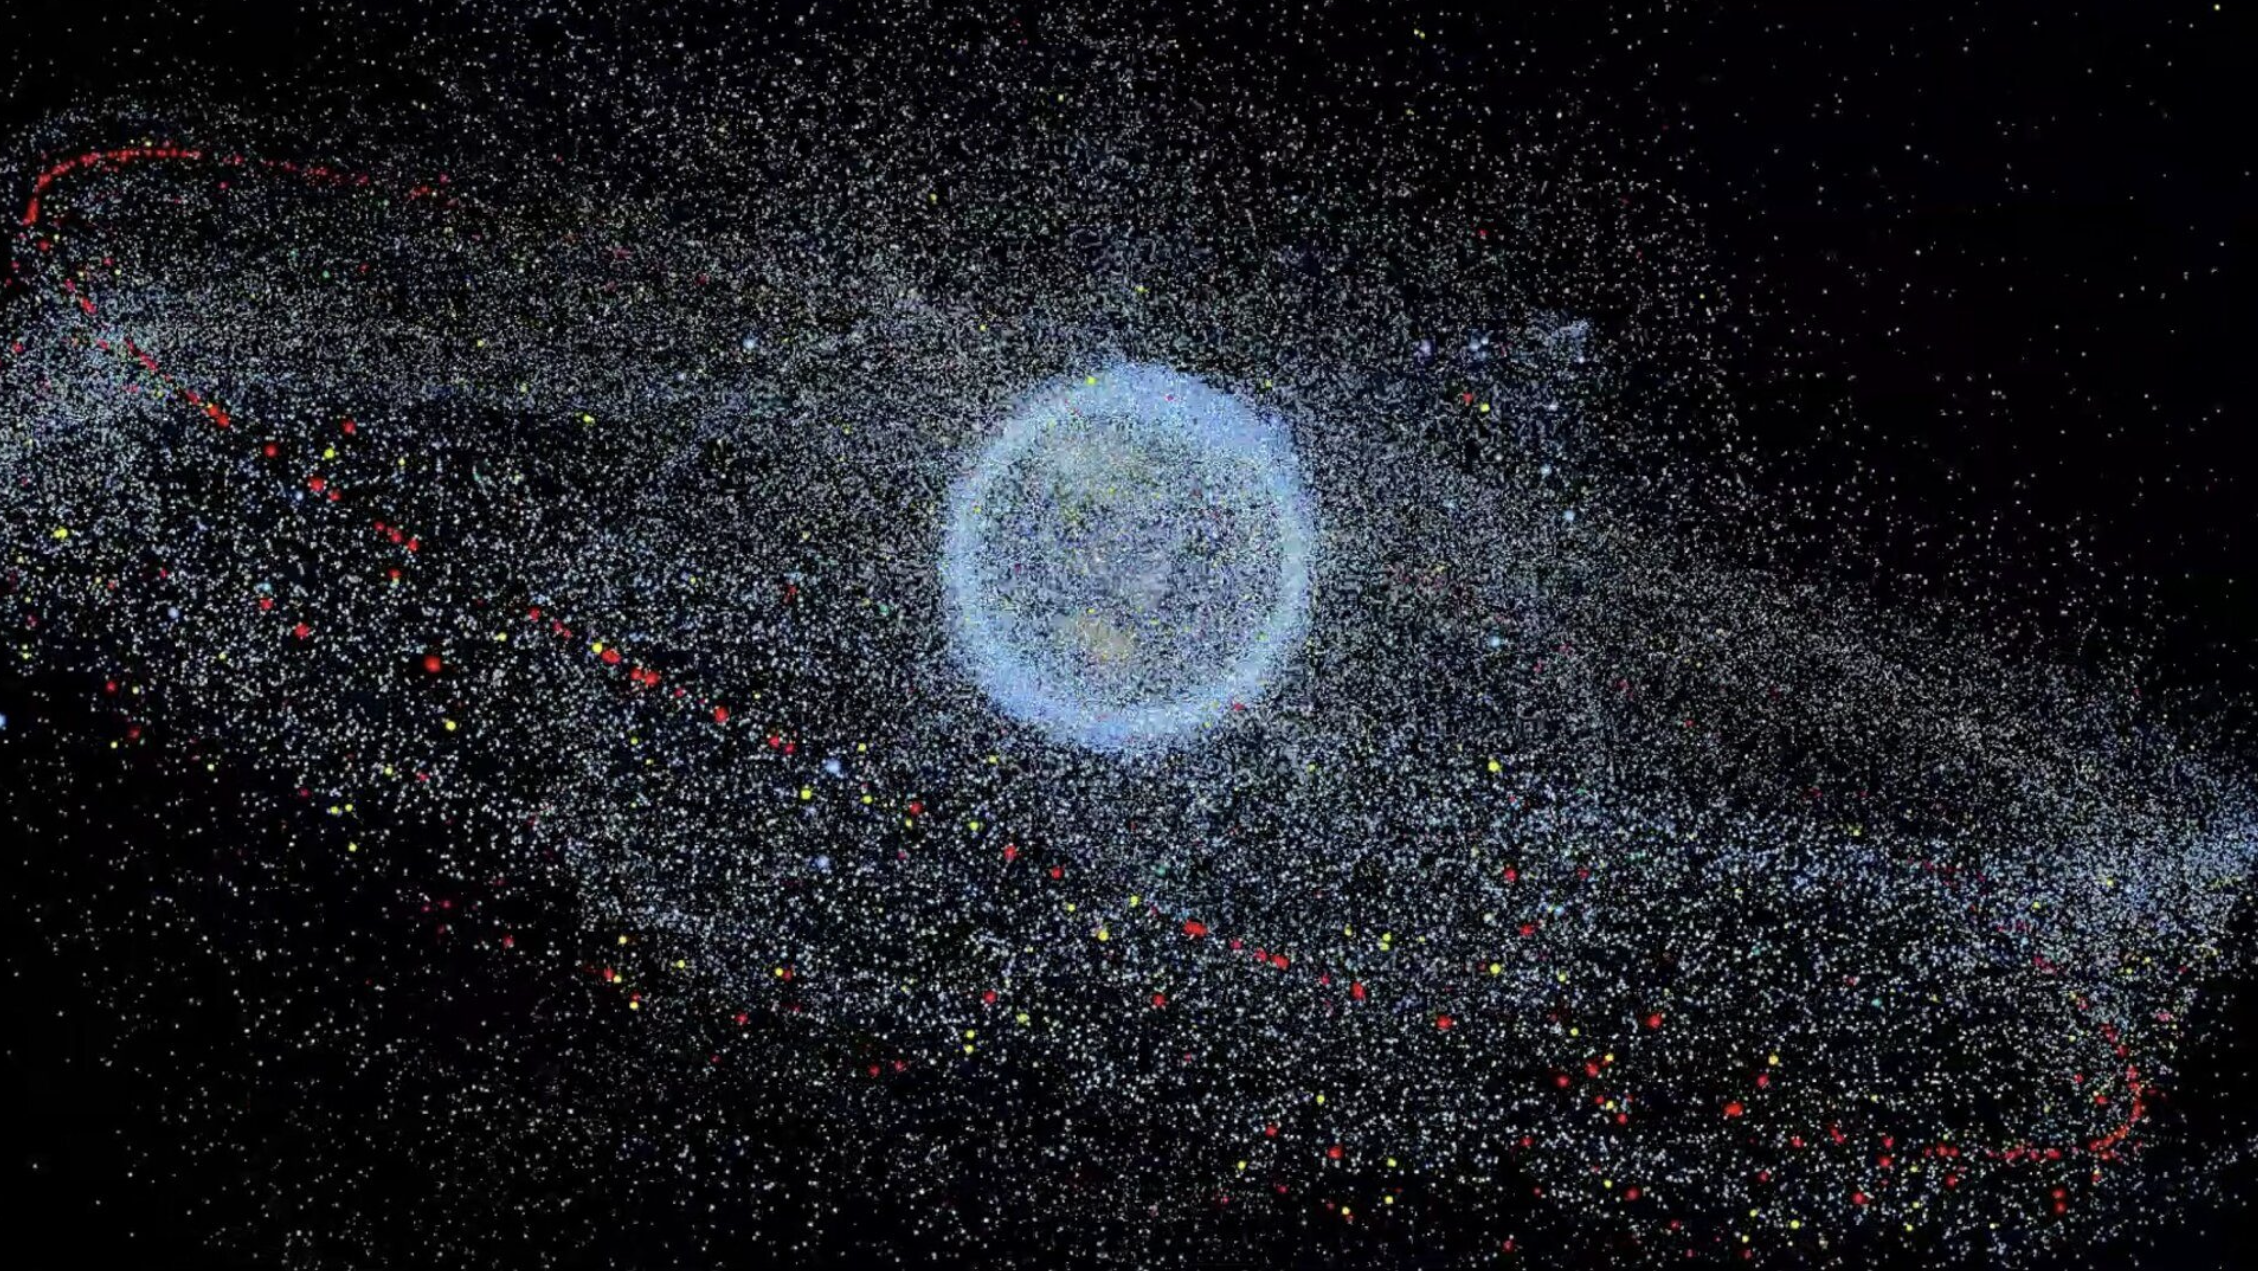
\includegraphics[width=0.8\linewidth]{images/All.png}
\end{center}

Heute prägen vor allem Satelliten den Alltag.

Sie ermöglichen:

\begin{itemize}
    \item Kommunikation
    \item Navigation
    \item Wettervorhersagen
    \item Erdbeobachtung
    \item globale Vernetzung
\end{itemize}

Mit dem Ausbau der Satelliteninfrastruktur
entsteht jedoch auch das Problem des Weltraumschrotts.

Raumfahrt wird dadurch zunehmend zu einer Frage
der nachhaltigen Nutzung orbitaler Infrastrukturen.

\subsection{Zentrale Erkenntnisse}

Die Geschichte der Raketentechnik ist keine reine Erfolgsgeschichte
technischer Innovation.

Sie zeigt:

\begin{itemize}
    \item Die enge Verbindung von Technik und Krieg
    \item Die politische Instrumentalisierung technischer Projekte
    \item Die Bedeutung symbolischer Macht im Kalten Krieg
    \item Die Entwicklung von spektakulären Missionen hin zu Infrastruktur
    \item Die zunehmende Rolle privater Akteure
\end{itemize}

Die zentrale These lautet:

Raketentechnik und Raumfahrt sind nicht nur technische Entwicklungen,
sondern gesellschaftliche Deutungsangebote.
Ihre Bedeutung verändert sich mit den politischen,
wirtschaftlichen und kulturellen Kontexten, in denen sie eingesetzt werden.